[84~v\textsuperscript{o}]
et fixitate, humiditate et siccitate, benignitate et corrosivitate, differentia; oleosa aut incombustibilia; \edtext{phlegmatica aut efficacia,}{\lemma{phlegmatica aut}\Bfootnote{\textit{(1)}\ virtute praedita \textit{(2)}\ efficacia, \textit{L}}}
denique salia, sulphura, spiritus\protect\index{Sachverzeichnis}{spiritus} produci posse.
Et errant qui tot
\edtext{diversas naturas inesse corporibus}{\lemma{diversas}\Bfootnote{%
\textit{(1)}\ partes %
\textit{(2)}\ naturas %
\textit{(a)}\ rebus %
\textit{(b)}\ inesse corporibus \textit{L}}} putant, quot rerum genera \edtext{eliciunt}{\lemma{genera}\Bfootnote{\textit{(1)}\ una e \textit{(2)}\ eliciunt. \textit{L}}}. Quaedam enim corpora recte tractata possunt \edtext{pene}{\lemma{}\Bfootnote{pene \textit{erg.} \textit{L}}} tota redigi in sal volatile, quae alia tractandi ratione quiddam partim fixum partim oleosum seu medium \edlabel{dabunt}dabunt.%
\edtext{}{{\xxref{dabunt}{difficultas}}\lemma{dabunt.}\Bfootnote{\textit{(1)}\ Sed regimine ignis redacto \textit{(2)}\ Facit [...] difficultas, \textit{L}}}%
\pend%
\pstart%
Facit haec regendi ignis difficultas,\edlabel{difficultas}
\edtext{ut Ars Chemica}{\lemma{ut}\Bfootnote{\textit{(1)}\ Chymia \textit{(2)}\ Ars Chemica \textit{L}}}
hactenus inter eas\edtext{\textso{ artes }fuerit,}{\lemma{\textso{artes}}\Bfootnote{\textit{(1)}\ fuerint \textit{(2)}\ fuerit, \textit{L}}} quarum effectus etiam omnibus exploratis non sunt in potestate,
\edtext{quas dicere possis\textso{ conjecturales }}{\lemma{}\Bfootnote{quas [...] \textso{conjecturales} \textit{erg. L}}}ut est Medica, et agricultoria, et
\edtext{nautica; Exempli causa, Opali artificiales}{\lemma{nautica;}\Bfootnote{\textit{(1)}\ unde Opalum  \textit{(a)}\ artificialem \textit{(b)}\ artificiales \textit{(2)}\ Exe \textit{(3)}\ Exempli causa,  \textit{(a)}\ Opalus \textit{(b)}\ Opali artificiales \textit{L}}}
saepe casu in officinis vitrariis producti sunt.
\edtext{At
% {\centering
% 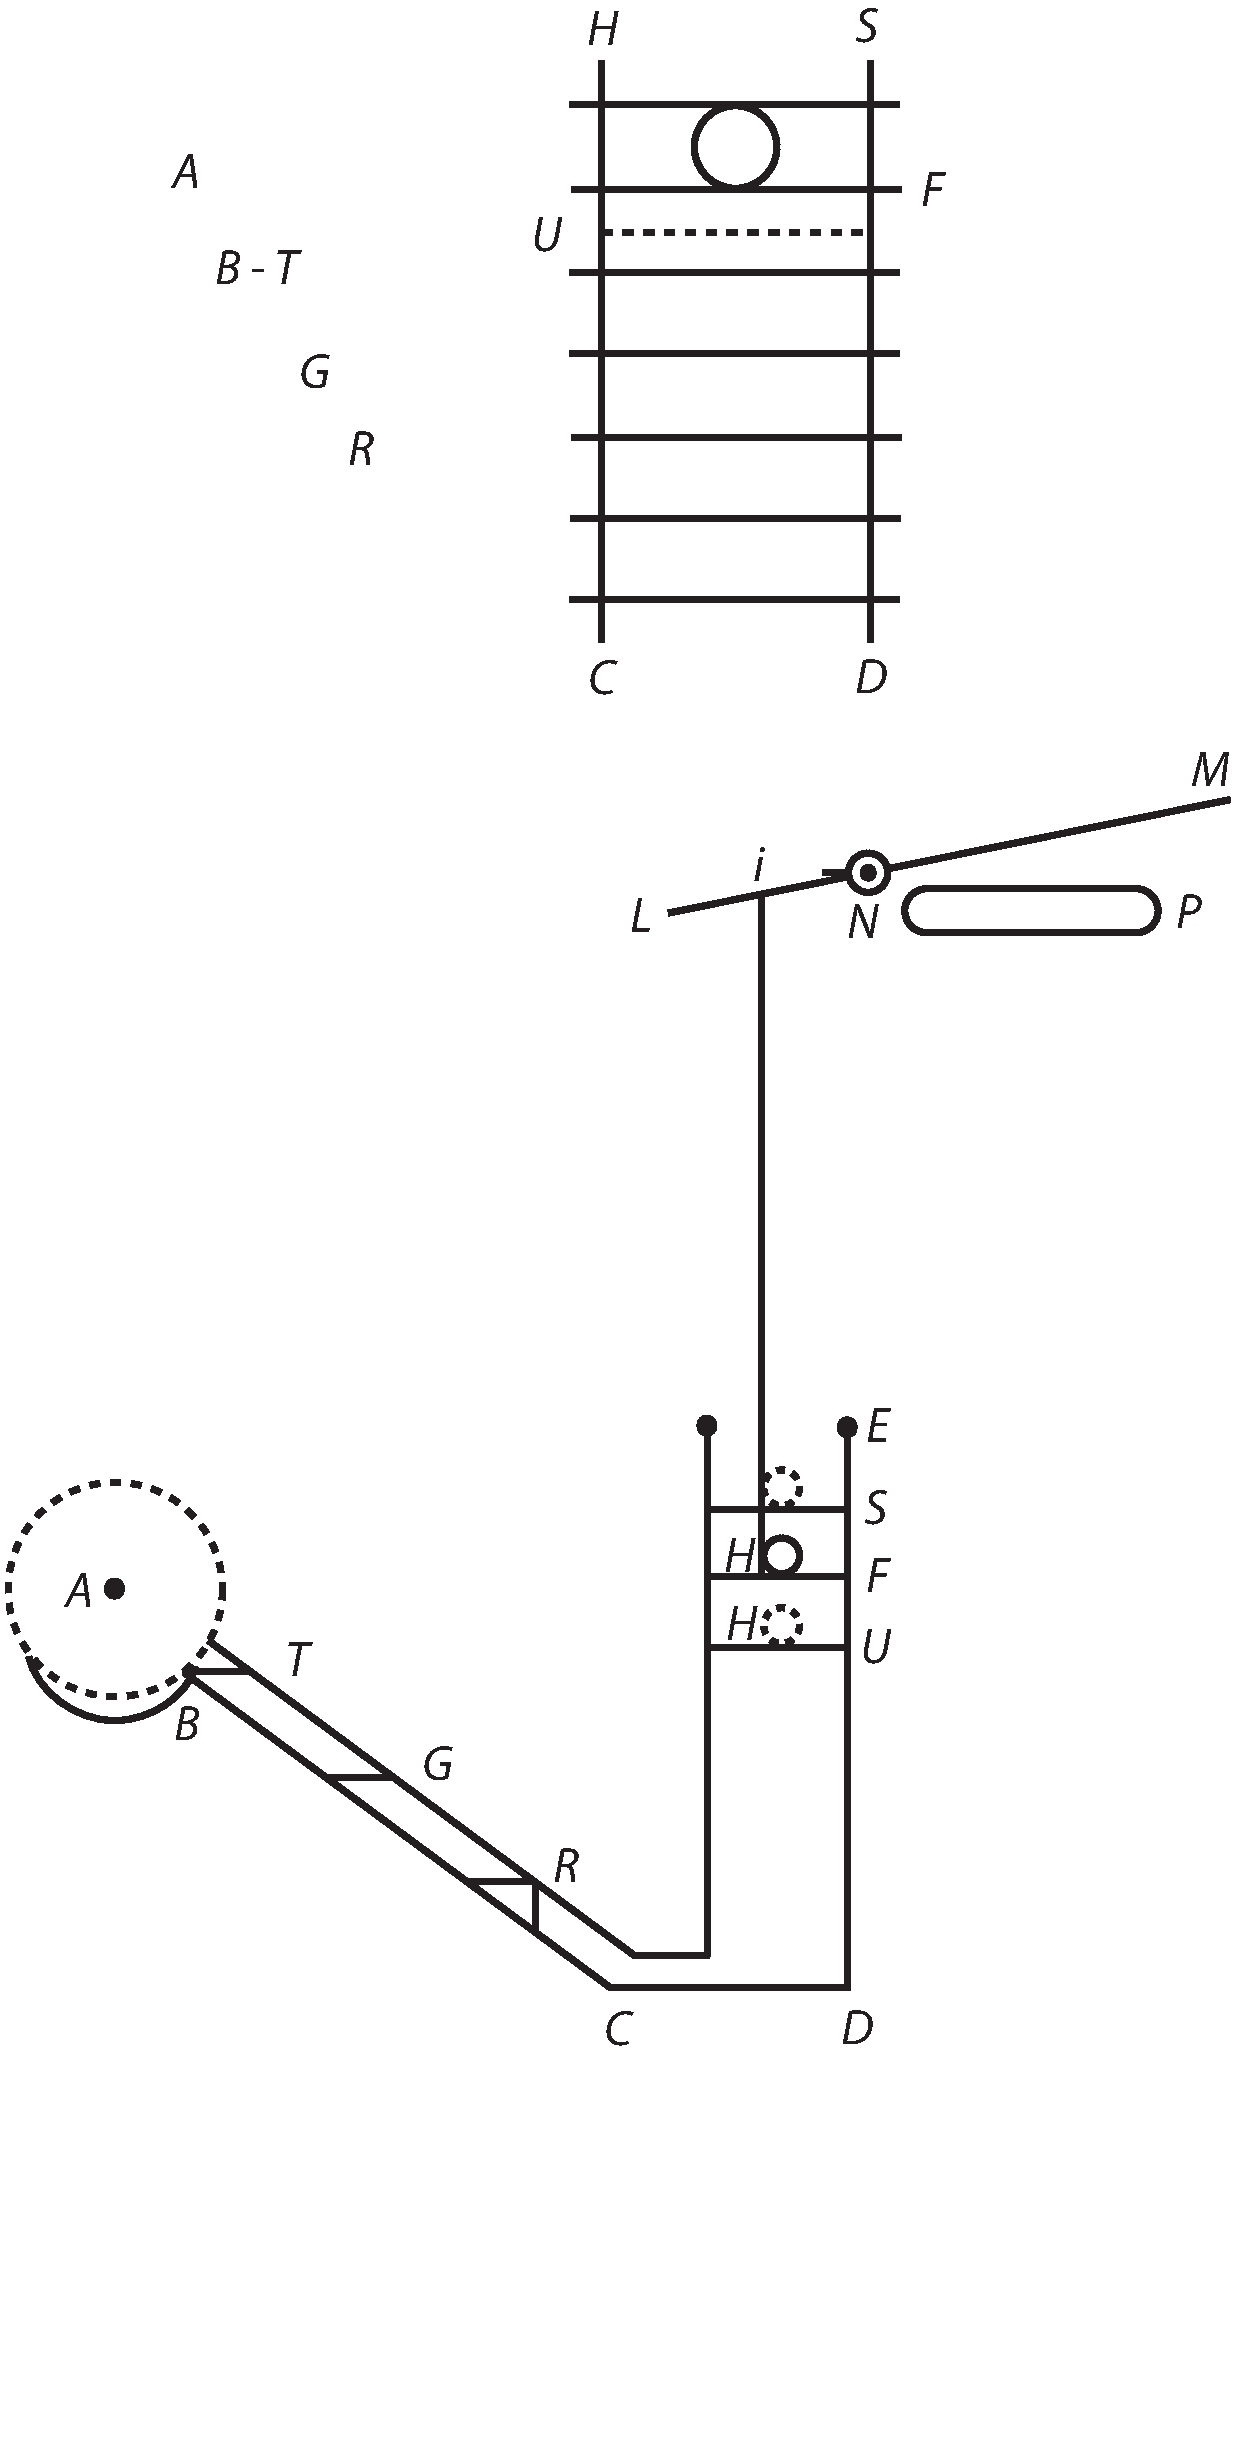
\includegraphics[width=0.65\textwidth]{images/lh03703_84v1u2.pdf}\\
% \rule[0mm]{45mm}{0mm}\textit{[Fig. 1, oberer Teil gestrichen]}
% }
regula certa faciendi cum velis, hactenus explorata non est.}{\lemma{At}\Bfootnote{\textit{(1)}\ qui \textit{(2)}\ in \textit{(3)}\ regulam certam faciendi invenerit \textit{(4)}\ regula [...] est. \textit{L}}}
Etsi ut obiter dicam notus mihi sit amicus,
\edtext{qui in eam}{\lemma{qui}\Bfootnote{\textit{(1)}\ possit \textit{(2)}\ in eam \textit{L}}}
post multa tentamenta tandem inciderit, quae calorum\protect\index{Sachverzeichnis}{calor} rationibus lumen non exiguum effundere potest, cum opalus intra se contineat pene omnes. Similiter
\edtext{Lacrymas vitri}{\lemma{Lacrymas vitri}\Cfootnote{Siehe hierzu \cite{00154}\textit{BH} I, S. 17f.
\cite{00061}\textsc{R. Hooke}, \textit{Micrographia}, London 1665, S. 33-44.}}
producere ex data gutta nemo hactenus artificum promittere potuit: vix enim paucae ex multis salvae evadunt.
\pend%
\pstart%
\edtext{Sed cum}{\lemma{Sed}\Bfootnote{\textit{(1)}\ si \textit{(2)}\ cum \textit{L}}}
datus ignis gradus prae$\langle$scribi$\rangle$
\edtext{poterit, Chemia erit in earum artium numero,}{\lemma{poterit,}\Bfootnote{\textit{(1)}\ chymia \textit{(2)}\ Chemia in earum artium numero erunt \textit{(3)}\ Chemia [...] numero, \textit{L}}}
quae sunt in artificis diligentis potestate, qualis est Architecturaria, et Pictoria et Scrinitria, et Tornatoria.
\pend%
\pstart%
Hoc fiet ergo
\edtext{aliquatenus (donec aliquis felicior rem ad majorem perfectionem deducat)}{\lemma{}\Bfootnote{aliquatenus [...] deducat) \textit{erg. L}}}
subtili \edtext{quadam applicatione Th$\langle$ermom$\rangle$etri}{\lemma{quadam}\Bfootnote{\textit{(1)}\ Thermo \textit{(2)}\ applicatione Th$\langle$ermom$\rangle$etri \textit{L}}}
ad Fornacem:\protect\index{Sachverzeichnis}{fornax}
\edtext{Sed Thermometri}{\lemma{Sed}\Bfootnote{\textit{(1)}\ Thermometris \textit{(2)}\ Thermometri \textit{L}}}
a caeteris $\langle$diversi$\rangle$,
caetera enim designant tantum,
hoc non solum $\langle$designa$\rangle$re
sed et \textso{facere} debet gradum caloris\protect\index{Sachverzeichnis}{calor} \edtext{datum[,] in usum deducendi}{\lemma{datum[,]}\Bfootnote{%
\textit{(1)}\ $\langle$in$\rangle$ praestandi \textit{(2)}\ in usum deducendi \textit{L}}}
hanc rationem $\langle$comm$\rangle$odissimam mihi videor reperisse.
\pend
\pstart
\edtext{$\langle$Es$\rangle$to Ampulla \textit{A} fornaci, eo in $\langle$loc$\rangle$o, ubi materia distillanda, digerendave etc. poni debet, implantata; ex%
}{\lemma{$\langle$Es$\rangle$to}\Bfootnote{\textbar \ Vas sive \textit{gestr.}\ \textbar \ Ampulla\ \textit{A} \textit{(1)}\ ex\ \textit{(2)}\ fornaci, [...] implantata; ex\ \textit{L}}} materia igni
\edtext{vel saltem calori\protect\index{Sachverzeichnis}{calor}}{\lemma{}\Bfootnote{vel saltem calori\protect\index{Sachverzeichnis}{calor} \textit{erg. L}}}
\edtext{resistente, facta.}{\lemma{resistente,}\Bfootnote{\textit{(1)}\ ut ferro, cupro, terra etc. facta \textit{(2)}\ facta. \textit{L}}}
Ex \edtext{hac Ampulla descendat}{\lemma{hac}\Bfootnote{\textit{(1)}\ descendat \textit{(2)}\ Ampulla descendat \textit{L}}}\hfill
\edtext{canna\hfill vitrea}{\lemma{canna}\Bfootnote{\textit{(1)}\ tenuis vitrea \textit{(2)}\ vitrea \textit{L}}}\hfill
\textit{BC}\hfill longa\hfill
\edtext{inclinataque}{\lemma{}\Bfootnote{inclinataque \textit{erg. L}}}\hfill
quantum\hfill satis\hfill est,\hfill et\hfill intrans\hfill in\hfill vas\hfill
\edtext{\textit{DE}}{\lemma{}\Bfootnote{\textit{DE} \textit{erg. L}}}
\pend
\vspace{2em}
\pstart%
\centering%
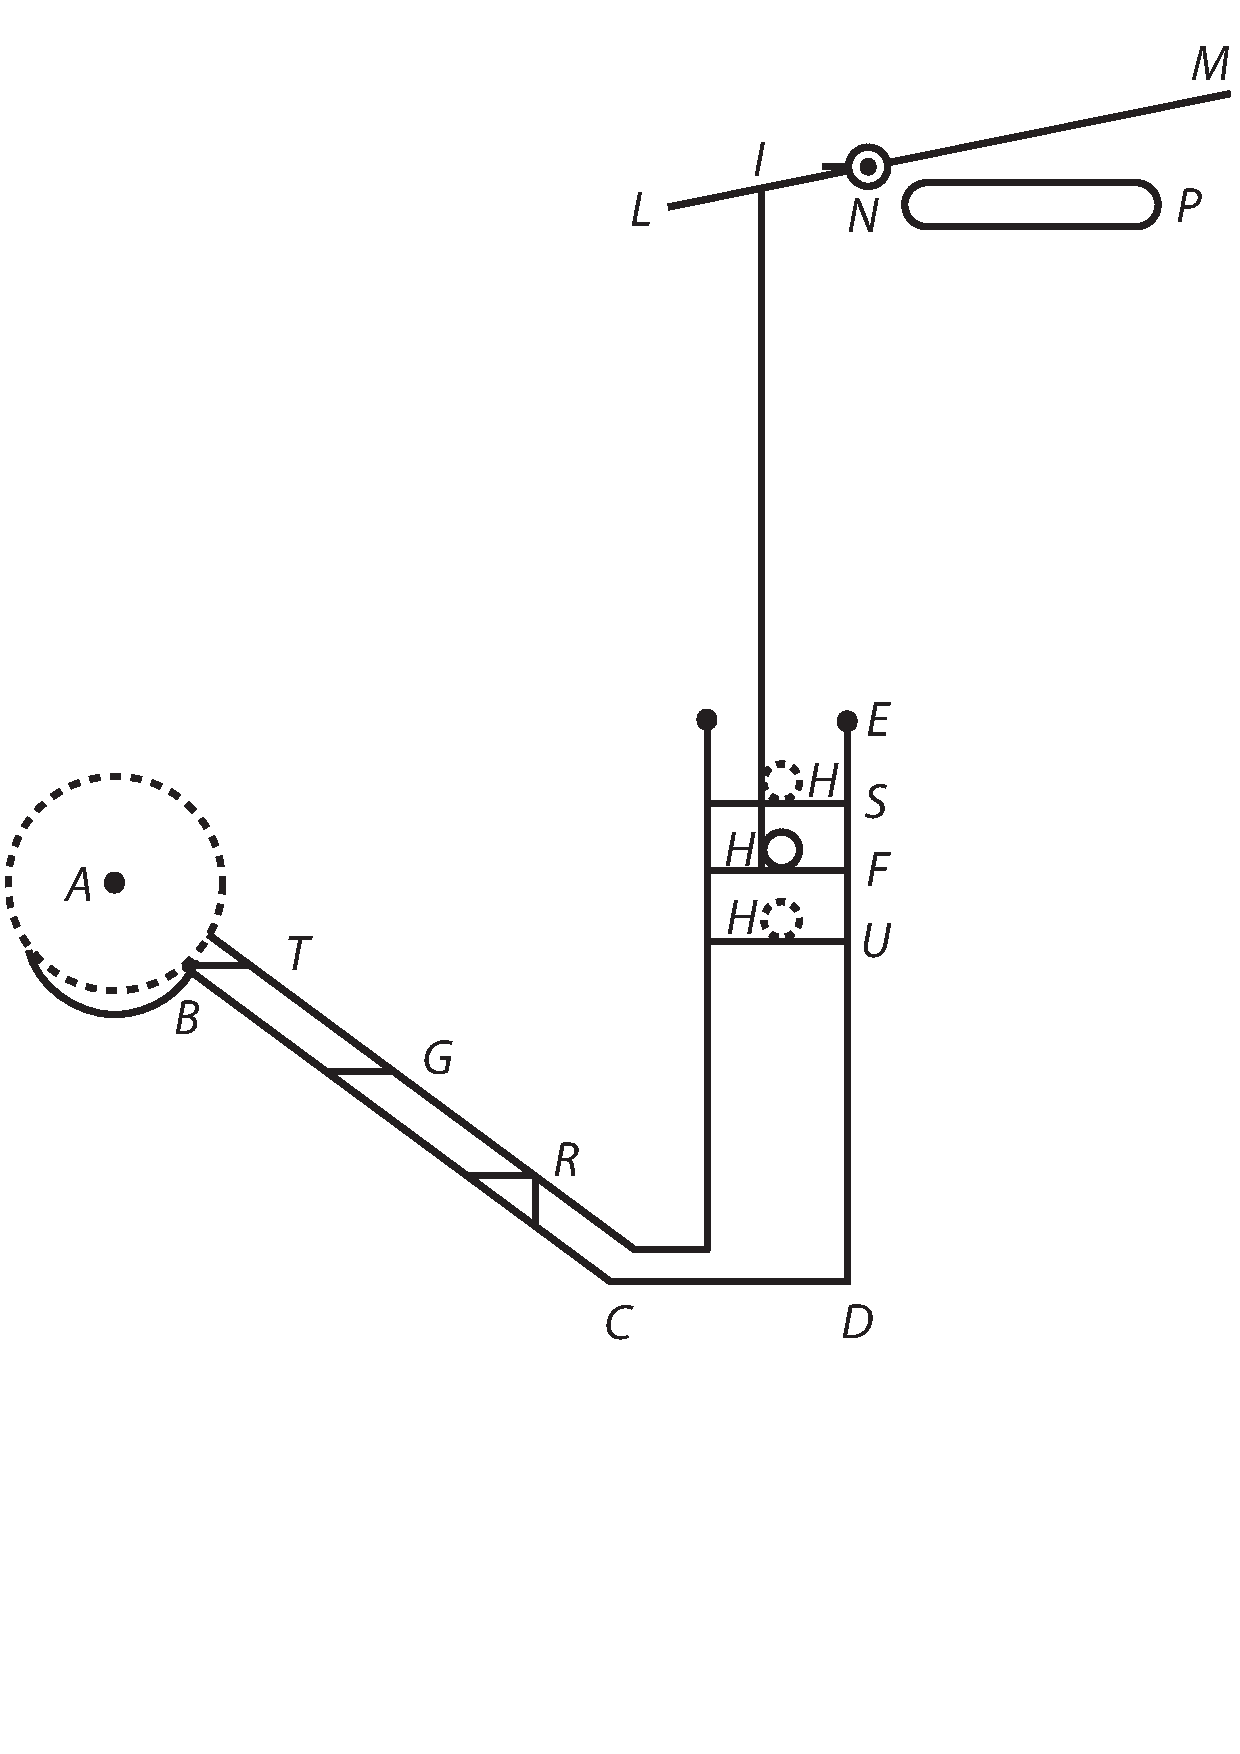
\includegraphics[width=0.68\textwidth]{images/lh03703_84v1.pdf}\\
\centering
[\textit{Fig. 1}]%
\edtext{}{\lemma{\hspace*{1,7mm}[\textit{Fig. 1}]}\killnumber\Cfootnote{Ein erster, gestrichener und hier nicht wiedergegebener Entwurf dieses Diagramms ist tlw. als Blindzeichnung ausgef\"{u}hrt.}}
\pend%%
\pstart%
\noindent liquore quodam (\phantom)\hspace{-1.2mm}ut aqua,
\edtext{vel argento vivo quod ideo commodius est, quia non aeque evaporat\phantom(\hspace{-1.2mm}) plenum usque ad \textit{F.}%
}{\lemma{vel}\Bfootnote{%
\textit{(1)}\ argentivo %
\textit{(2)}\ argento vivo %
\textbar\ quod [...] evaporat \textit{erg.}\ \textbar\ %
\phantom(\hspace{-1.2mm}) %
\textit{(a)}\ plenum %
\textit{(b)}\ refertum \textit{DE} %
\textit{(c)}\ plenum usque ad \textit{F.} %
\textit{L}}}
ita ut hujus liquoris pars in cannae partem, quanta satis
\edtext{est, \textit{CG} vi aequilibrii ascendat,}{\lemma{est,}\Bfootnote{\textit{(1) }\ ascendat \textit{(2)}\ \textit{CG} [...] ascendat, \textit{L}}}
\edtext{quousque aeris jam inclusi raritas permittit.}{\lemma{quousque}\Bfootnote{\textit{(1)}\ per aerem jam inclusum potest \textit{(2)}\ aeris [...] permittit. \textit{L}}}
\pend%
% \newpage% PR: Rein provisorisch !!!
% \vspace*{2.5em}% PR: Rein provisorisch !!!
% \pstart%
% \centering%
% 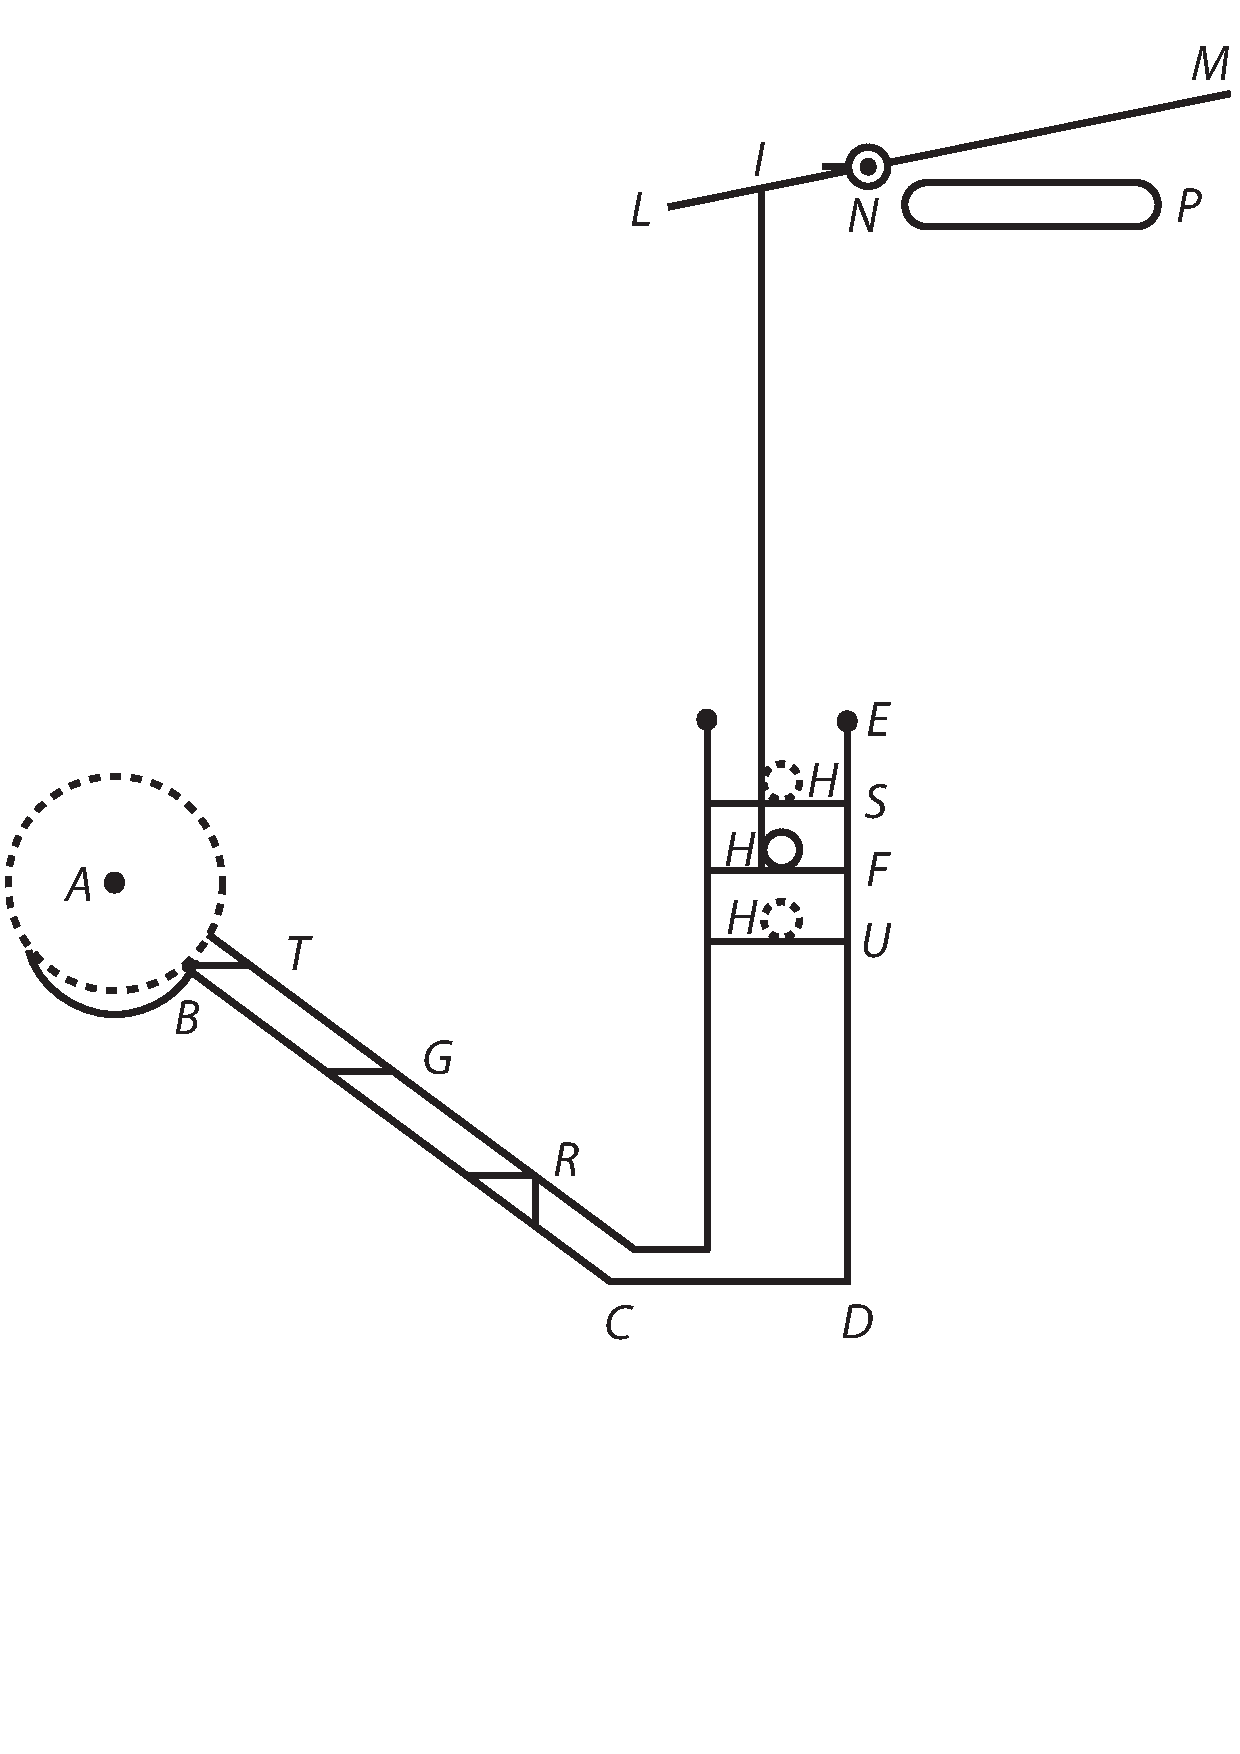
\includegraphics[width=0.7\textwidth]{images/lh03703_84v1.pdf}%
% \vspace*{0.5em}% PR: Rein provisorisch !!!
% \newline%
% [\textit{Fig. 1}]%
% \edtext{}{\lemma{\hspace*{1,7mm}[\textit{Fig. 1}]}\killnumber\Cfootnote{Ein erster, gestrichener und hier nicht wiedergegebener Entwurf dieses Diagramms ist tlw. als Blindzeichnung ausgef\"{u}hrt.}}
% \pend%
% \vspace*{1.0em}% PR: Rein provisorisch !!!
% \newpage% PR: Rein provisorisch !!!
\pstart%
\edtext{In superficie liquoris in vase \textit{DE} natet}{\lemma{In}\Bfootnote{\textit{(1)}\ liquore vasis \textit{DE} natet \textit{(2)}\ \textit{DF} liquore vasis, \textit{(3)}\ superficie [...] natet \textit{L}}}
corpus \edtext{quoddam \textit{H} eo}{\lemma{quoddam}\Bfootnote{\textit{(1)}\ eo \textit{(2)}\ \textit{H} eo \textit{L}}}
liquore \edtext{levius ex}{\lemma{}\Bfootnote{levius\ \textbar\ (v.g. \textit{(1)}\ lignum \textit{(2)}\ suber in aqua, plumbum in Hydrargyro) \textit{gestr.}\ \textbar\ ex \textit{L}}}
\edtext{quo ascendat}{\lemma{quo}\Bfootnote{\textit{(1)}\ prodeat \textit{(2)}\ ascendat \textit{L}}}
\edtext{baculus \textit{HI} annexus laminae ferreae \textit{LM}}{\lemma{baculus \textit{HI}}\Bfootnote{\textit{(1)}\ attingens laminam \textit{(2)}\ annexus [...] \textit{LM} \textit{L}}}
mobili circa centrum \textit{N} et
\edtext{imminenti Registro}{\lemma{imminenti}\Bfootnote{\textit{(1)}\ foramin \textit{(2)}\ Registro \textit{L}}}
seu aperturae
\edtext{sive Respiraculo}{\lemma{sive Respiraculo}\Bfootnote{\textit{erg. L}}}
fornacis\protect\index{Sachverzeichnis}{fornax} \textit{P}.
\pend%
%\newpage% PR: Rein provisorisch !!!
% \vspace*{2.5em}% PR: Rein provisorisch !!!
%\vspace*{1.0em}% PR: Rein provisorisch !!!
% \newpage% PR: Rein provisorisch !!!
\count\Afootins=1100
\pstart%
Hic qui nunc est status ponatur esse debitus, seu desideratus, is ergo semper manebit (quamdiu ignis sufficiens in fornace\protect\index{Sachverzeichnis}{fornax} supererit.)
Aer \edtext{enim in Ampulla \textit{A} ulterius,%
}{\lemma{enim in}\Bfootnote{%
\textit{(1)}\ fornace %
\textit{(2)}\ Ampulla \textit{A} %
\textit{(a)}\ ultra %
\textit{(b)}\ ulterius, %
\textit{ L}}}
calore\protect\index{Sachverzeichnis}{calor}
\edtext{rarefactus, in liquorem (aquam aut mercurium) in canna \textit{BC} deprimet}{\lemma{rarefactus,}\Bfootnote{\textit{(1)}\ partem mercurii\ \textbar\ \textit{GC} \textit{erg.}\ \textbar\
 \textit{(a)}\ ex canna \textit{(b)}\ ex canna \textit{BC} deprimet \textit{(2)}\ in liquorem (aquam aut mercurium) \textit{(a)}\  \textit{GC} \textit{(b)}\ in canna \textit{BC} deprimet \textit{L}}}
ex \edtext{altitudine}{\lemma{}\Bfootnote{altitudine \textit{erg. L}}}
\textit{GC} \edtext{in \textit{RC}. Ergo residuum liquoris, (differentia inter \textit{GC} et \textit{RC}) deprimetur in}{\lemma{in \textit{RC}.}\Bfootnote{\textit{(1)}\ Is ergo ascendet in \textit{(2)}\ Ergo [...] deprimetur in \textit{L}}}
\edtext{vas}{\lemma{}\Afootnote{\textit{Am Rand:}
Nota:\textsuperscript{[a]} posse abesse\textsuperscript{[b]} [Ampullam] \textit{A} et totum aerem esse in canna.
Potest canna in spiras intorta esse, eaeque spirae possunt esse in vase quodam cupreo grandi aqua pleno.
Quo facto poterunt vitreae esse, poterunt a destructione conservari,\textsuperscript{[c]} habebunt eundem semper caloris\protect\index{Sachverzeichnis}{calor} gradum ubique.
Metuendum ne inter vibrationes in\textsuperscript{[d]} medio quoddam aequilibrium eligatur. Sed et hae ultro citroque reciprocationes reddent calorem\protect\index{Sachverzeichnis}{calor} inaequalem, nec nisi dimidium ejus, toto tempore, gradus dati.
Ergo efficiendum ut magis semper decrescat quam crescat calor\protect\index{Sachverzeichnis}{calor}.
Si \textit{HI} baculus sit propior centro laminae laminaque longior, ita aequilibrium subdividet incrementa in duas partes inaequales, ex quibus praedominabitur pars renitens mutationi, seu minima erit mutatio.
Ita minima mutatio maximam resistentiam experietur.
Et tempore reciprocationis calor\protect\index{Sachverzeichnis}{calor} erit partim magnus partim nullus, aut parvus.
Manebit ergo prior, si justa proportio assignetur.\vspace{2mm}\\%
{\footnotesize%
\textsuperscript{[a]} Nota: \textit{(1)}\ potest \textit{(2)}\ posse \textit{L}
\hspace{5mm}\textsuperscript{[b]} abesse \textit{(1)}\ vas \textit{(2)}\ Ampulla \textit{L ändert Herausgeber}
\hspace{5mm}\textsuperscript{[c]}~conservari, \textit{(1)}\ retinebunt \textit{(2)}\ habebunt \textit{L}
\hspace{5mm}\textsuperscript{[d]} in \textit{erg. L}\vspace{-8mm}}}}
%%
liquore refertum, ac propterea liquor ascendet in vase ex \textit{F} in \textit{S}.
Ergo et corpus \textit{H} natans in liquore.
Ergo et baculus \textit{HI} elevabit brachium laminae \textit{LN} eodem ergo tempore deprimet brachium laminae oppositum \textit{NM}
\edtext{id est operculum}{\lemma{}\Bfootnote{id est operculum \textit{erg. L}}}
ac proinde magis quam ante occludet Registrum seu foramen \textit{NP}.
Quo facto calor\protect\index{Sachverzeichnis}{calor}
% \edtext{minuetur,}{\lemma{minuetur,}\Bfootnote{\textit{ (1) }\ ac proinde